\documentclass{article}

\usepackage{alltt}
\renewcommand{\ttdefault}{txtt}

\usepackage{graphicx}
\newcommand{\HRule}{\rule{\linewidth}{0.5mm}}

\usepackage{soul}


\sethlcolor{yellow}

\usepackage{listings}
\usepackage{hyperref}
\usepackage{amsmath}


\usepackage{color}
\definecolor{lightgray}{rgb}{.9,.9,.9}
\definecolor{darkgray}{rgb}{.4,.4,.4}
\definecolor{purple}{rgb}{0.65, 0.12, 0.82}

\lstdefinelanguage{JavaScript}{
  keywords={typeof, new, true, false, catch, function, return, null, catch, switch, var, if, in, while, do, else, case, break},
  keywordstyle=\color{blue}\bfseries,
  ndkeywords={class, export, boolean, throw, implements, import, this},
  ndkeywordstyle=\color{darkgray}\bfseries,
  identifierstyle=\color{black},
  sensitive=false,
  comment=[l]{//},
  morecomment=[s]{/*}{*/},
  commentstyle=\color{purple}\ttfamily,
  stringstyle=\color{red}\ttfamily,
  morestring=[b]',
  morestring=[b]"
}

\lstset{ %
  language=JavaScript,
  extendedchars=true,
  basicstyle=\footnotesize\ttfamily,
  showstringspaces=false,
  showspaces=false,
  numbers=left,
  numberstyle=\footnotesize,
  numbersep=9pt,
  tabsize=2,
  breaklines=true,
  showtabs=false,
  captionpos=b
}

\let\oldsection\section 
\renewcommand{\section}{\clearpage\oldsection} 

\begin{document}

\begin{titlepage}

\begin{center}


% Upper part of the page

\includegraphics[width=0.20\textwidth]{./sjsu.jpg}\\[1cm]    

\textsc{\LARGE San Jose State University}\\[1.5cm]

\textsc{\Large Network \& Protocols Project 2}\\[0.5cm]


% Title
\HRule \\[0.6cm]
{ \huge \bfseries Simulation of Ethernet Medium Access Control protocols}\\[0.4cm]

\HRule \\[1.5cm]

% Author and supervisor
\begin{center}
Alexandre \textsc{Joseph} \\
Audric \textsc{Albaret} \\
Nicolas \textsc{Roux} 
\end{center}
\vfill

% Bottom of the page
{\large \today}

\end{center}

\end{titlepage}


\setcounter{tocdepth}{2}

\tableofcontents

\clearpage

\section{Introduction}

The network \& protocol course that we attempt teach us foundations and
advanced aspects of networking such as data link network and MAC, packet
switching, internetworking, end-to-end protocols and also congestion
control and resource allocation.

As a part of this course, we need to do a team project allowing us to
apply notions that we have studied. The goal of the project is to do
simulation of a Medium Access Control (MAC) protocol.

Moreover this simulation will allow us to evaluate the performances of
the used medium access control protocol.

The medium access control protocol is a sub-layer of the data link layer
(layer 2) specified in the seven-layer OSI model and the four layer
TCP/IP model (layer 1). It provides addressing and channel access
control mechanisms making communication between different hosts
possible within a multiple network.

The MAC protocols performs many function such as receiving and
transmitting frames, appending check sequence to frame, discarding
malformed frames or even backoff functions.

Many MAC protocols exists, such as Ethernet, Wifi or Token Ring. Each of
this protocols have it own multiple access protocols taking advantage of
the used medium constraints or topology. For example, the Ethernet
protocol use CSMA/CD, the Wifi protocol use CSMA/CA and the Token Ring
protocol use the Token bus.

For the purpose of this project, we focused on only one medium access
control protocol.


\section{Ethernet protocols}

Ethernet protocols refer to a family of computer networking technologies
used in Local Area Network. Developed by Xerox in 1973, it have been
commercially introduced in 1980. Since its release, it has retained a
good degree of compatibility.

With the time, Ethernet has been standardized in IEEE 802.3 and has
replaced most of the other wired LAN technologies. Some of this features
such as 48-bit MAC address and Ethernet frame format have influenced
other networking protocols.

The Ethernet system consists of three basic elements:

\begin{enumerate}
    \item The physical medium used to carry Ethernet signal between
    computers.
    \item A set of medium access control rules embedded in each Ethernet
    interface that allow multiple computers to fairly arbitrate access
    to the shared Ethernet channel
    \item An  Ethernet frame that consists of a standardized set of bits
    used to carry data over the system.
\end{enumerate}

Each host that is using Ethernet operates independently of all other
station on the network, there is no central controller. All hosts are
connected the same link (the medium). Therefor before sending data
on this link, they need to listen the channel to make sure nobody else
is using it. The medium access control mechanism used by Ethernet use a
system called Carrier Sense Multiple Access with Collision Detection
(CSMA/CD).

As Ethernet is a widely used standard and it design robustness has been
proved and influenced many other protocols, it appear to be very
interesting to study this subject and to try to simulate this protocol.
We will moreover do some performance evaluation on the Ethernet
protocols to measure and compare some parameters like delay, delay
jitter and throughput.


\section{Simulator technologies}

The project instructions has no specific requirement regarding the
implementation technologies used. This let us the choice in the language
used to simulate the chosen networking protocol.

Many implementations of Ethernet have been done in C mainly because it
is the most learned language in Computer Science course and for some
implementation for performance reasons. Therefor it seemed interesting
for us to do the simulator using other technologies.

The simulator require some interactions with the user, for the input
parameters and the output informations. As user experience matter, a
graphical and easy to use interface is a big advantage. Having a
graphical user interface will make easer performances evaluation and
statistics with automatic plotting.

The use of JavaScript for the computation part and HTML5 with CSS3
appear to be a smart choice. Those technologies are very popular nowadays
and many improvement has been done in the past year on it. The reasons
of this popularity are mainly due to the ease of use of those
technologies. Indeed every one can execute a simple script or view a web
page with it wen browser. There is no need to install many tools such as
compiler, libraries and so on. In addition, thanks to advanced
frameworks such as JQuery, development and cross-compatibility have
become much easier.
Moreover all the modern browser such as Chrome, Firefox or Internet
Explorer are evolving very quickly to support more and more features and
performances of JavaScript engine has never been so good. We
can now execute huge script in a browser without experiencing latency.


\section{Carrier Sense Multiple Access with Collision Detection}

TODO: Explain algorithm with exponential backoff and implementation.

\begin{figure}[h!]
  \centering
    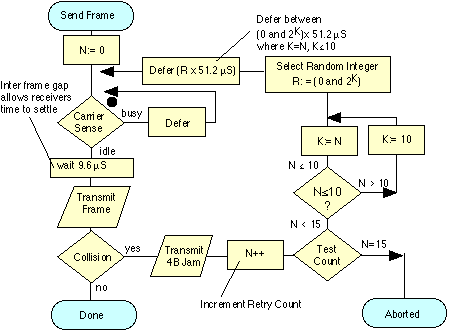
\includegraphics[width=\textwidth]{figures/csmacd.png}
  \caption{CSMA/CD algorithm representation}
\end{figure}


\section{Design concepts}

``... with proper design, the features come cheaply. This approach is
arduous, but continues to succeed.''
\begin{flushright}
\emph{Dennis Ritchie}, C and Unix inventor
\end{flushright}

\huge{This is a draft of the design concepts}

Objects:

\begin{description}
    \item[Paquito] orchestrator
    \item[Packet] packet representation
    \item[Host] host representation
    \item[Link] link representation
\end{description}

Hosts try to send until it have packet to send.
Hosts notify link that there are sensing. Then when sensing time is elapsed,
orchestrator will call the send method. If the boolean saying that the
link is idle have not been set to false the packet is sent.
If the link was not idle, a new sense request is sent to the link and so
on.
Every time a host is sending a packet, for each host on the link between
sender and receiver, the link will be set to in use when the signal is
under the adaptor and reset to idle when the packet is transmitted.
If a host try to send a packet will another one is sending a jam signal
is sent to all the host and all the packet, traffic notification and
sensing are discarded. Host will wait a random time between 0 and 2 pow
K with K incrementing by one each consecutive jam signal until 15. When a
host successfully send a packet, K is reset to 0.


\section{Synchronous traffic}

TODO: Introduce synchronous traffic.

Packet arrival and inter arrival time are all uniform and deterministic.

\begin{description}
    \item Arrival process : packet size / bandwidth ( packets/sec)
    \item Traffic load = packet arrival time rate * packet size
    \item Average packet delay = transmission time for one packet
    \item Delay Variance = 0 because intervals are equal.
    \item Thoughput = $\frac{number of byte sent}{total time}$
\end{description}

TODO: Explain constant bit rate


\section{Asynchronous traffic}

TODO: Introduce asynchronous traffic.

\begin{description}
    \item Arrival process : $ \frac{e^{b} \cdot b^{k}}{k!}$ (Poisson distribution)
    \item Traffic load = packet arrival time rate  (Poisson distribution : $ \frac{e^{b} \cdot b^{k}}{k!}$) $\times$ packet size (Exponential distribution : $\lambda \cdot e^{ \lambda \cdot t}$)

	\begin{description}  
        \item b = $\lambda \cdot$t
        \item t is used to define the interval 0 to t   
        \item $\lambda$ is the total average arrival rate in packets
        \item k is the total number of packets in the interval 0 to t
   	\end{description}

    \item Average packet delay = $\overline{x} = \dfrac{1}{n} \sum_{i=1}^{n} x_{i}$
    \item Delay Variance = $ V(X) = \dfrac{1}{n} \sum_{i=1}^{n} x_{i}^{2} - \overline{x}$

    	\begin{description}
            \item X : Delay
            \item n = number of packets
            \item $x_{i} = delay for packet number \times i$
            \item $\overline{x} = average packet delay$
       	\end{description}

    \item Thoughput = $\frac{number of byte sent}{total time}$
\end{description}

\subsection{Poisson process}

TODO: Expose concept and implementation



\section{Performance analysis}

TODO: Do some benchmark and comment results.


\section{List of references}

\begin{description}
    \item Chapter 2 of the textbook by Peterson and Davie
    \item The set of handout on simulation provided.
    \item \href{http://mathworld.wolfram.com/PoissonDistribution.html}{http://mathworld.wolfram.com/PoissonDistribution.html}
    \item \href{http://www.erg.abdn.ac.uk/~gorry/eg3561/lan-pages/csma-cd.html}{http://www.erg.abdn.ac.uk/~gorry/eg3561/lan-pages/csma-cd.html}
\end{description}


\end{document}
